%!TEX root = ../main.tex

\section{Dynammic Programming}

\subsection{Station Placement Problem}

Image there is a bunch of towns $t_1, ..., t_n$ in a train line, where
$t_i \in \mathbb{N}$. Now you want to put $k$ stations to minimize
the maximum distance that a resident of any town has to commute to the nearest station. 

How many towns should be served by the last station? In the DP
approach, we try all possible answers. For example, we could set the
last station to serve the last town, or we could set the last station
to serve the last two towns, etc. More generally, suppose the last
station serves towns $t_i, t_{i + 1}, ..., t_n$. Then we should put
the station at the mean of the two extreme towns it is serving, i.e.,
at $\frac{t_i + t_n}{2}$. Note that then the cost of any person in the
extreme towns going to station at $\frac{t_i + t_n}{2}$ is
$\frac{t_n - t_i}{2}$ (see Figure~\ref{fig:stations}).


\begin{figure}[hpt]
    \centering
    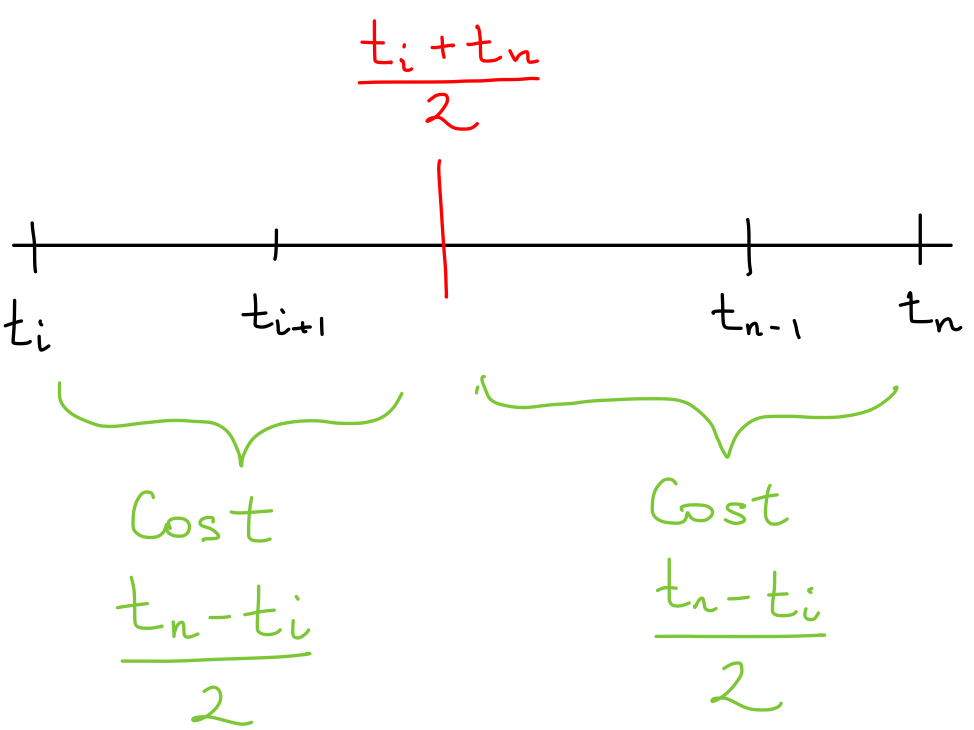
\includegraphics[width=0.5\textwidth]{figures/stations.jpeg}
    \caption{Where to put the station when considering the last 
    $n - i + 1$ towns.}
    \label{fig:stations}
\end{figure}

Let's introduce some notation. The cost $C(n, k)$ is the cost of 
serving towns $t_1, ..., t_n$ with $k$ stations. More generally,
the cost $C(i, j)$ is the cost of serving towns $t_1, ..., t_i$
through $j$ stations.

If we decide to make the last station serve towns $t_i$ through
$t_n$, then 

$$
C(n, k) = \max \Big (\frac{t_n - t_i}{2}, \; C(i - 1, k - 1) \Big )
$$

Since we don't know the best $i$, we can write 

$$
C(n, k) = \min_{i = 1 \to n} \max \Big (\frac{t_n - t_i}{2}, \; C(i -
1, k - 1) \Big )
$$

This defines a recurrence relation or a tree (see Figure~
\ref{fig:dp-tree}).

\begin{figure}[hpt]
    \centering
    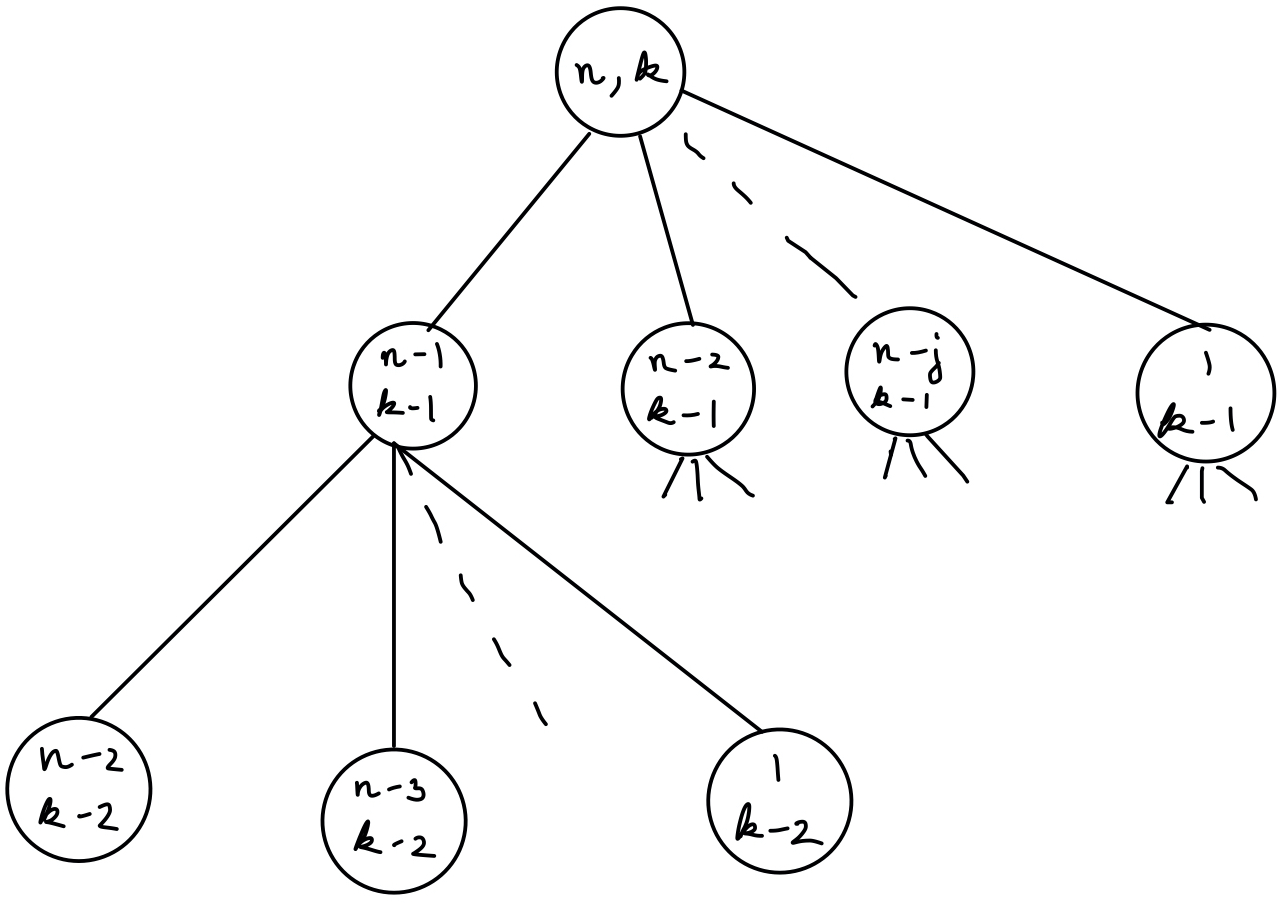
\includegraphics[width=0.5\textwidth]{figures/dp-tree.jpeg}
    \caption{Subproblems in the stations problem.}
    \label{fig:dp-tree}
\end{figure}

\subsubsection{Naive Algorithm}

Compute $C(n, k)$ exactly as in the recurrence above.

\begin{algorithm}
\caption{Algorithm to calculate $C(n, k)$}
\begin{algorithmic}
\IF{$n$ is 0}
\STATE{return 0}
\ENDIF
\IF{$k$ is 1}
\STATE{return $\frac{t_i - t_1}{2}$}
\ENDIF
\STATE{$currmin = \infty$}
\FOR{$i = 1$ to $n$}
\STATE{$C = \max \Big (\frac{t_n - t_i}{2}, \; C(i - 1, k - 1) \Big)$}
\IF{$currmin < C$}
\STATE{$currmin = C$}
\ENDIF
\ENDFOR
\STATE{return $currmin$}
\end{algorithmic}
\end{algorithm}

This recursive algorithm runs in exponential time. What will save us
is that in fact there are not too many distinct subproblems. The
problem in this algorithm is that we are solving the same subproblem
repeatedly.

\subsubsection{Memoization (Top Down) Algorithm}

The idea is to maintain solutions to subproblems in an array instead
of computing them repeatedly, so every subproblem is solved only once.

\begin{algorithm}
\caption{Algorithm to calculate $C(n, k)$}
\begin{algorithmic}
\REQUIRE{$A$ is a 2d array shared between all recursive calls}
\IF{$A[n][k]$ is not null}
\STATE{return $A[n][k]$}
\ENDIF
\IF{$n$ is 0}
\STATE{update $A[n][k]$}
\STATE{return 0}
\ENDIF
\IF{$k$ is 1}
\STATE{update $A[n][k]$}
\STATE{return $\frac{t_i - t_1}{2}$}
\ENDIF
\STATE{$currmin = \infty$}
\FOR{$i = 1$ to $n$}
\STATE{$C = \max \Big (\frac{t_n - t_i}{2}, \; C(i - 1, k - 1) \Big)$}
\IF{$currmin < C$}
\STATE{$currmin = C$}
\ENDIF
\ENDFOR
\STATE{update $A[n][k]$ to be $currmin$}
\STATE{return $currmin$}
\end{algorithmic}
\end{algorithm}

We have $nk$ subproblems, each taking $O(n)$ time, which leads to a
$O(n^2k)$ algorithm.

\subsection{Binary Strings in Unary Representation}

For this problem, given a number $n$ in unary, count the number of
binary strings of length $n$ that do not contain the pattern $11$.
For instance, 3 is represented as 111 in unary. The bitstrings
000, 001, 010, 100, 101 do not contain the pattern, so the answer is
5.

\begin{remark}
    The reason we give $n$ in unary is because if we give it in binary
the algorithm will take exponential time.
\end{remark}

Say a string is valid if it does not contain the pattern 11. Then the
top level question is to count the number of valid strings of length
$n$ ending in 0 and similarly count the number of valid strings of
length $n$ ending in 1. What can we say about a valid bitstring of
length $n$? We have two cases

\begin{itemize}
    \item Case 1: The bitstring ends in 0. Then the first $n - 1$
    bits can be any valid bitstring of length $n - 1$.
    \item Case 2: The bitstring ends in 1. Then the first $n - 1$
    bits can be any valid bitstring of length $n - 1$ ending with a 0.
\end{itemize}

Let $S_1(n)$ be the number of valid strings of length $n$ ending in 1,
and let $S_0(n)$ be the number of valid strings of length $n$ ending
in 0, so that $S(n) = S_0(n) + S_1(n)$. The recurrence then becomes


\begin{align*}
    S_1(n) &= S_0(n - 1) \\
    S_0(n) &= S(n - 1) = S_0(n- 1) + S_1(n - 1) \\
    S(n) &= 2S_0(n - 1) + S_1(n - 1) \\
\end{align*}

This follows a Fibonacci sequence, and can be solved with dynamic
programming.

\subsection{Subsequences}

\begin{definition}
    Given a sequence of positive integers $a_1, ..., a_n$, a subsequence
is a sequence $a_{i_1}, ..., a_{i_k}$, where $i_1 < ... < i_k$.     
\end{definition}

\begin{definition}
    We say a subsequence is increasing if $a_{i_1} < ... < a_{i_k}$.
\end{definition}

Suppose you are given a sequence 9, 5, 27, 2, 6, 1, 8, 3, 11.
An increasing subsequence is 5, 6, 8, 11.

\begin{remark}
    (Aside). Given any sequence of length $n^2 + 1$, it either has
    an increasing subsequence of length $n + 1$ or a decreasing
    subsequence of length $n + 1$. This is a generalization of the
    pigeonhole principle.
\end{remark}

Let $a_1, ..., a_n$.
We will now try to find the longest increasing
subsequence. A wrong top level question you could ask is: is $a_n$ in
the longest increasing subsequence? 

Let $\text{Best}(i, l) = x$ if the increasing sequence of length $l$
in the prefix of $a_1, ..., a_i$ with the smallest ending number
ends in $x$. Take the sequence 100, 1, 2, 3, 4, 8.
Then $\text{Best}(1, 1) = 100$, $\text{Best}(2, 1) = 1$,
$\text{Best}(2, 2) = \infty$. 















